\section{Paging: Faster Translations (TLBs)}

%------------------------------------------------
\begin{frame}{The Problem: Paging Is Slow}

\begin{itemize}
    \item Paging needs a large amount of mapping information,
          generally stored in \textbf{physical memory}.
    \item Every virtual address requires an \textbf{extra memory lookup}
          for the translation, before each instruction fetch, load or store.
    \item Help comes from the OS's old friend: the \textbf{hardware}.
\end{itemize}

\begin{block}{The Crux: How to Speed Up Address Translation}
How can we speed up address translation, and generally avoid the extra
memory reference that paging seems to require? What hardware support is
required? What OS involvement is needed?
\end{block}

\end{frame}

%------------------------------------------------
\begin{frame}{Translation-Lookaside Buffer (TLB)}

\begin{itemize}
    \item Part of the chip's \textbf{memory-management unit (MMU)}.
    \item A \textbf{hardware cache} of popular virtual-to-physical
          address translations (a better name: \textit{address-translation cache}).
    \item On each memory reference, the hardware first checks the TLB:
    \begin{itemize}
        \item if the translation is there, it is performed quickly,
              \textbf{without consulting the page table};
        \item otherwise, the page table (which has all translations) is used.
    \end{itemize}
    \item Because of their performance impact, TLBs in a real sense
          \textbf{make virtual memory possible}.
\end{itemize}

\end{frame}

%------------------------------------------------
\begin{frame}{TLB Basic Algorithm}

\begin{columns}[T]

\column{0.38\textwidth}
\small
\begin{itemize}
    \item Simple linear page table; \textbf{hardware-managed} TLB.
    \item Extract the VPN and look it up in the TLB.
    \item \textbf{TLB hit}: build the physical address from the PFN
          and the offset (after protection checks).
    \item \textbf{TLB miss}: access the page table, update the TLB,
          and \textbf{retry the instruction}.
\end{itemize}

\column{0.60\textwidth}
\begin{figure}
    \centering
    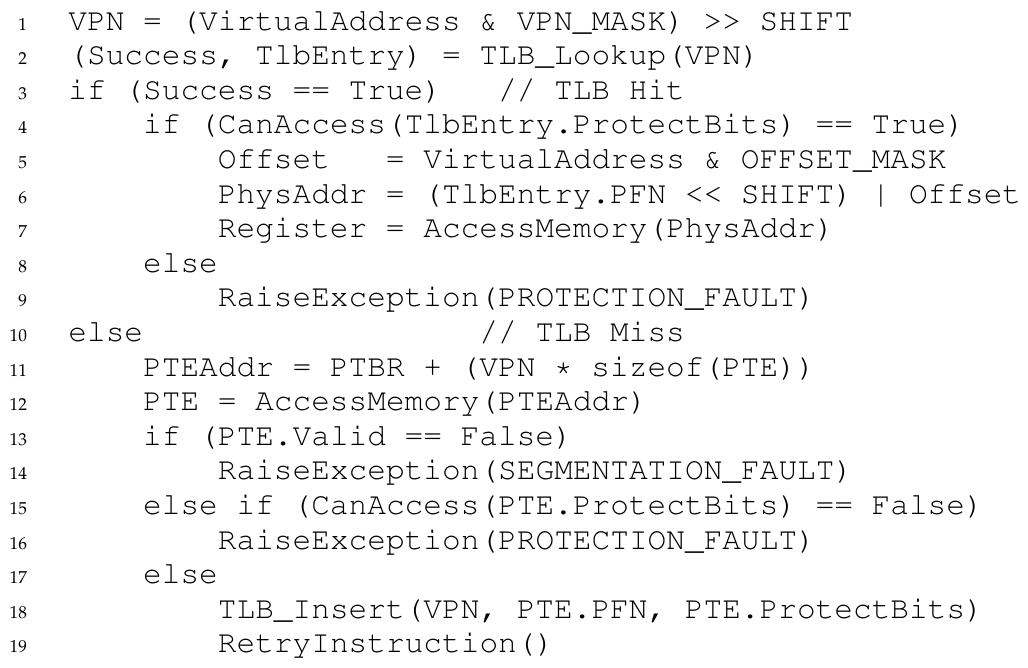
\includegraphics[width=1.0\linewidth]{figs/chapter-19/figure-19.1.png}
    \caption*{Source: chapter page 2.}
    \label{fig:figure-19.1}
\end{figure}

\end{columns}

\end{frame}

%------------------------------------------------
\begin{frame}[fragile]{Example: Accessing an Array}

\begin{columns}[T]

\column{0.55\textwidth}
\begin{itemize}
    \item Array of 10 4-byte integers starting at virtual address 100.
    \item 8-bit virtual address space, 16-byte pages:
          4-bit VPN and 4-bit offset.
\end{itemize}

\begin{lstlisting}[style=CStyle]
int i, sum = 0;
for (i = 0; i < 10; i++) {
    sum += a[i];
}
\end{lstlisting}

\begin{itemize}
    \item Result: miss, hit, hit, miss, hit, hit, hit, miss, hit, hit.
    \item \textbf{Hit rate} $= 7/10 = 70\%$.
\end{itemize}

\column{0.38\textwidth}
\begin{figure}
    \centering
    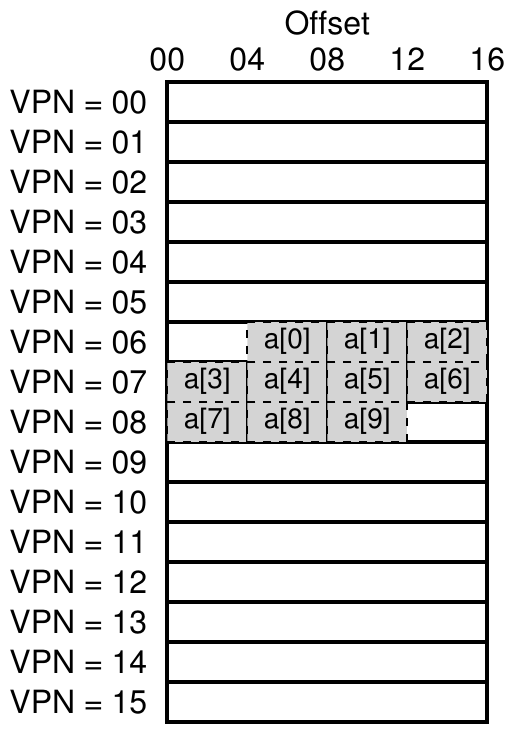
\includegraphics[height=0.5\textheight]{figs/chapter-19/figure-19.2.png}
    \caption*{Source: chapter page 4.}
    \label{fig:figure-19.2}
\end{figure}

\end{columns}

\end{frame}

%------------------------------------------------
\begin{frame}{Locality and the TLB}

\begin{itemize}
    \item \textbf{Spatial locality}: elements packed tightly into pages;
          only the first access to each page misses.
    \item \textbf{Page size} matters: with 32-byte pages, even fewer misses;
          with typical 4KB pages, a single miss per page of accesses.
    \item \textbf{Temporal locality}: re-accessing the array soon after
          would yield all hits (if the TLB is big enough).
\end{itemize}

\begin{block}{Tip: Use Caching When Possible}
Caches exploit temporal and spatial locality by keeping copies in small,
fast on-chip memory. Why not bigger caches? A fast cache must be
\textbf{small}, due to physical constraints.
\end{block}

\end{frame}

%------------------------------------------------
\begin{frame}{Who Handles the TLB Miss?}

\begin{columns}[T]

\column{0.46\textwidth}
\begin{itemize}
    \item \textbf{Hardware} (CISC, e.g., Intel x86):
    \begin{itemize}
        \item knows where page tables are (\textbf{PTBR}/CR3) and their format;
        \item ``walks'' the page table and updates the TLB.
    \end{itemize}
    \item \textbf{Software} (RISC, e.g., MIPS, SPARC):
    \begin{itemize}
        \item hardware just raises an exception;
        \item a \textbf{trap handler} in the OS updates the TLB with
              privileged instructions.
    \end{itemize}
\end{itemize}

\column{0.52\textwidth}
\begin{figure}
    \centering
    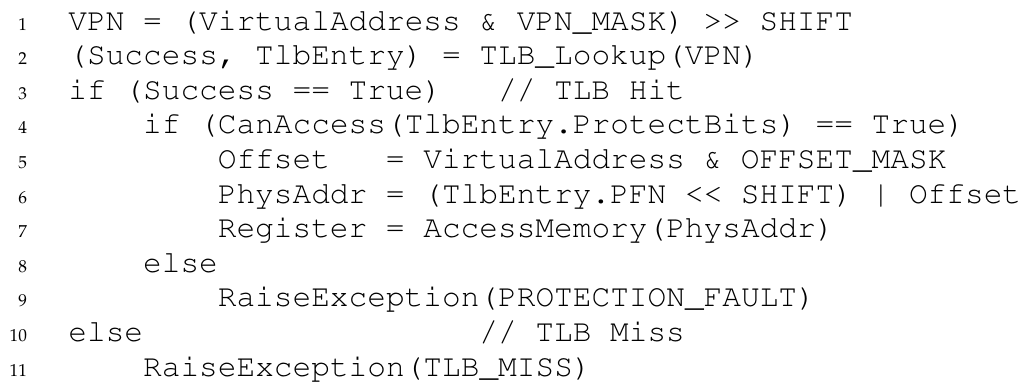
\includegraphics[width=1.0\linewidth]{figs/chapter-19/figure-19.3.png}
    \caption*{Source: chapter page 6.}
    \label{fig:figure-19.3}
\end{figure}

\end{columns}

\end{frame}

%------------------------------------------------
\begin{frame}{Software-Managed TLB: Details}

\begin{itemize}
    \item The return-from-trap must resume at the
          \textbf{instruction that caused the trap} (retry),
          not at the next one as in a system call.
    \item Avoid an \textbf{infinite chain of TLB misses}:
    \begin{itemize}
        \item keep miss handlers in unmapped physical memory, or
        \item reserve \textbf{wired} TLB entries for the handler code.
    \end{itemize}
    \item Advantages: \textbf{flexibility} (any page-table data structure)
          and \textbf{simplicity} of the hardware.
\end{itemize}

\begin{block}{Aside: RISC vs. CISC}
CISC: many powerful instructions. RISC: few simple primitives as compiler
targets. Today both kinds of processors can be made to run fast.
\end{block}

\end{frame}

%------------------------------------------------
\begin{frame}{TLB Contents}

\begin{itemize}
    \item Typically 32, 64 or 128 entries; \textbf{fully associative}
          (any translation can be anywhere, searched in parallel).
    \item Entry: \quad \texttt{VPN \;|\; PFN \;|\; other bits}
    \item Other bits: \textbf{valid} bit, \textbf{protection} bits,
          address-space identifier, dirty bit, \ldots
\end{itemize}

\begin{alertblock}{Aside: TLB valid bit $\neq$ page-table valid bit}
\begin{itemize}
    \item \textbf{PTE invalid}: page not allocated; access traps and the
          process is likely killed.
    \item \textbf{TLB entry invalid}: simply no valid translation cached there
          (e.g., at boot, or after a context switch).
\end{itemize}
\end{alertblock}

\end{frame}

%------------------------------------------------
\begin{frame}{TLB Issue: Context Switches}

\begin{itemize}
    \item TLB translations are valid only for the \textbf{running process}.
    \item Example: VPN 10 maps to PFN 100 (P1) and to PFN 170 (P2).
\end{itemize}

\begin{center}
\footnotesize
\begin{tabular}{cccc}
\toprule
VPN & PFN & valid & prot \\
\midrule
10 & 100 & 1 & rwx \\
--- & --- & 0 & --- \\
10 & 170 & 1 & rwx \\
--- & --- & 0 & --- \\
\bottomrule
\end{tabular}
\end{center}

\begin{block}{The Crux: How to Manage TLB Contents on a Context Switch}
The translations of the last process are not meaningful to the
about-to-be-run process. What should the hardware or OS do?
\end{block}

\end{frame}

%------------------------------------------------
\begin{frame}{Solutions: Flush or ASID}

\begin{columns}[T]

\column{0.50\textwidth}
\small
\begin{itemize}
    \item \textbf{Flush} the TLB on each context switch
          (set all valid bits to 0):
    \begin{itemize}
        \item works, but each process incurs misses when it runs again.
    \end{itemize}
    \item \textbf{Address Space Identifier (ASID)}:
    \begin{itemize}
        \item like a PID with fewer bits (e.g., 8);
        \item TLB holds translations of several processes;
        \item OS sets a privileged register with the current ASID.
    \end{itemize}
\end{itemize}

\column{0.46\textwidth}
\footnotesize
\begin{center}
\begin{tabular}{ccccc}
\toprule
VPN & PFN & valid & prot & ASID \\
\midrule
10 & 100 & 1 & rwx & 1 \\
--- & --- & 0 & --- & --- \\
10 & 170 & 1 & rwx & 2 \\
\bottomrule
\end{tabular}

\vspace{0.5cm}

\textbf{Sharing} (e.g., code pages): \\[0.2em]
\begin{tabular}{ccccc}
\toprule
VPN & PFN & valid & prot & ASID \\
\midrule
10 & 101 & 1 & r-x & 1 \\
--- & --- & 0 & --- & --- \\
50 & 101 & 1 & r-x & 2 \\
\bottomrule
\end{tabular}
\end{center}

\end{columns}

\end{frame}

%------------------------------------------------
\begin{frame}{Issue: Replacement Policy}

\begin{block}{The Crux: How to Design TLB Replacement Policy}
Which TLB entry should be replaced when we add a new TLB entry?
Goal: minimize the miss rate (increase the hit rate).
\end{block}

\begin{itemize}
    \item \textbf{LRU} (least-recently-used): exploits locality in the
          memory-reference stream.
    \item \textbf{Random}: simple and avoids corner cases.
    \begin{itemize}
        \item A loop over $n+1$ pages with a TLB of size $n$:
              LRU misses on \textbf{every} access; random does much better.
    \end{itemize}
    \item Policies are studied in detail later (swapping pages to disk).
\end{itemize}

\end{frame}

%------------------------------------------------
\begin{frame}{A Real TLB Entry: MIPS R4000}

\begin{figure}
    \centering
    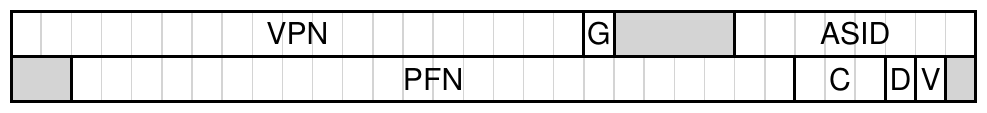
\includegraphics[width=0.85\linewidth]{figs/chapter-19/figure-19.4.png}
    \caption*{Source: chapter page 11.}
    \label{fig:figure-19.4}
\end{figure}

\begin{itemize}
    \item 32-bit address space, 4KB pages; \textbf{19-bit VPN}
          (user addresses use half of the space); up to \textbf{24-bit PFN}
          (64GB of memory).
    \item \textbf{G}: global bit (ASID ignored); 8-bit \textbf{ASID};
          \textbf{C}: coherence bits; \textbf{D}: dirty; \textbf{V}: valid.
\end{itemize}

\end{frame}

%------------------------------------------------
\begin{frame}{MIPS TLB Management}

\begin{itemize}
    \item \textbf{Wired} register: tells the hardware how many TLB slots
          to reserve for the OS (e.g., for the TLB miss handler).
    \item Privileged instructions to update the TLB:
    \begin{itemize}
        \item \texttt{TLBP}: probes for a translation;
        \item \texttt{TLBR}: reads an entry into registers;
        \item \texttt{TLBWI}: replaces a specific entry;
        \item \texttt{TLBWR}: replaces a random entry.
    \end{itemize}
    \item They \textbf{must be privileged}: a user process modifying the TLB
          could take over the machine.
\end{itemize}

\begin{block}{Question}
What should the OS do if more than 256 ($2^8$) processes are running?
\end{block}

\end{frame}

%------------------------------------------------
\begin{frame}{Summary}

\begin{itemize}
    \item A small, dedicated on-chip TLB makes most translations fast;
          performance is almost as if memory were not virtualized.
    \item \textbf{Exceeding the TLB coverage}: accessing more pages than fit
          in the TLB causes many misses.
    \begin{itemize}
        \item Solution: \textbf{larger pages} for key data structures
              (e.g., in a DBMS).
    \end{itemize}
    \item TLB access can become a pipeline bottleneck with
          \textbf{physically-indexed caches};
          \textbf{virtually-indexed caches} help, but add complexity.
\end{itemize}

\begin{block}{Tip: RAM Isn't Always RAM (Culler's Law)}
Randomly accessing an address space beyond the TLB coverage can lead to
severe performance penalties.
\end{block}

\end{frame}

%------------------------------------------------
\begin{frame}{Homework (Measurement)}

\begin{columns}[T]

\column{0.52\textwidth}
\begin{itemize}
    \item Write \texttt{tlb.c}: touch one integer per page of a large array,
          for \texttt{NUMPAGES} pages, timing many trials.
    \item Look for \textbf{jumps in cost} to infer TLB levels and sizes.
    \item Watch out for: timer precision, compiler optimizations,
          \textbf{pinning} the thread to one CPU, array initialization
          (demand zeroing).
\end{itemize}

\column{0.44\textwidth}
\begin{figure}
    \centering
    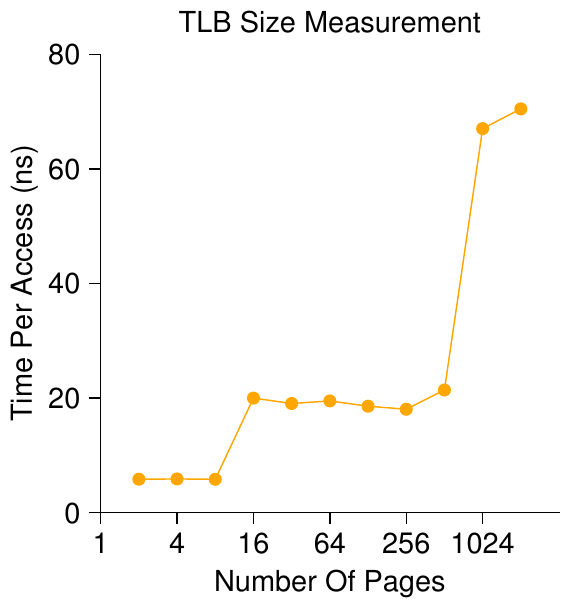
\includegraphics[width=0.95\linewidth]{figs/chapter-19/figure-19.5.png}
    \caption*{Source: chapter page 15.}
    \label{fig:figure-19.5}
\end{figure}

\end{columns}

\end{frame}
